\chapter{Check routines for reinforced concrete}
\section{Introduction}
This chapter describes the routines that can be used to check the design following the specifications of different design codes.

\section{Verification of RC sections}

\subsection{Sections definition}



\subsection{Limit State at Failure under normal stresses verification}

\subsubsection{lanzaCalculoTNFromXCData}
This function carries out the verification of the limit state at failure under nornal stresses. It takes as input the internal forces and bending moments calculated for the shell elements for every ULS combinations, the sections definition and the interaction diagrams to be employed.

The function returns two files with the verification results:
{\tt outputFileName.py}: XC file that assigns each shell element the capacity factor (worst-case) {\tt FCC} calculated for reinforcement in directions 1 and 2, together with the concomitant axial force and bending moments {\tt N My Mz}.
{\tt outputFileName.py}: \LaTeX\  file containing a table with the following items:

\begin{center}
\begin{tabular}{ccccccc}
\multicolumn{7}{l}{\textbf{Section 1}} \\
\\
Element & Section & ULS & Axial & Bending & Bending & Capacity \\
number  & name & name & force NCP1 & moment MyCP1 & moment MzCP1 & factor FCCP1 \\
\hline
\multicolumn{7}{l}{\ldots\ \ldots\ \ldots} \\
\\
\multicolumn{7}{l}{\textbf{Section 2}} \\
\\
Element & Section & ULS & Axial & Bending & Bending & Capacity \\
number  & name & name & force NCP2 & moment MyCP2 & moment MzCP2 & factor FCCP2 \\
\hline
\multicolumn{7}{l}{\ldots\ \ldots\ \ldots} \\
\\

\end{tabular}
\end{center}

\begin{figure}[h]
\centering
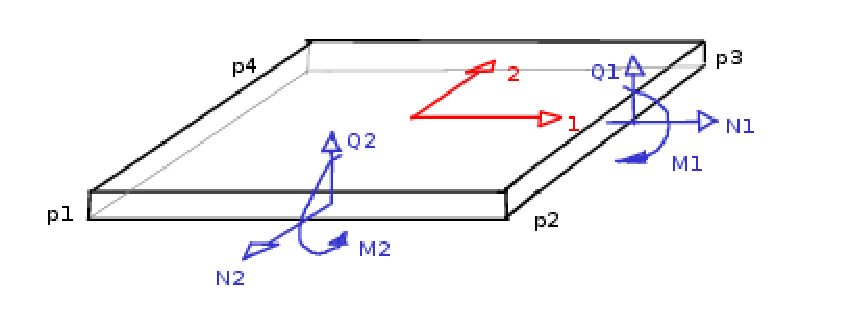
\includegraphics[width=100mm]{materials/figures/signosEsfuerzos}
\caption{Positive directions of forces and moments in shell elements}\label{shell_forces_moments}
\end{figure}

 
\begin{verbatim}
from materials.xLamina import calculo_tn
calculo_tn.lanzaCalculoTNFromXCData(preprocessor,analysis,intForcCombFileName,outputFileName, 
mapSectionsForEveryElement,mapSectionsDefinition, mapInteractionDiagrams)
\end{verbatim}
\begin{paramFuncTable}
\preprocessor{} \\
\analysis{} \\
\intForcCombFileName{ULS under normal stresses}{ULS}\\
\outputFileName{}\\
\mapSectionsForEveryElement{} \\
\mapSectionsDefinition{} \\
\mapInteractionDiagrams{} \\
\end{paramFuncTable}


\subsection{Limit State of Failure due to shear verification}
This function carries out the verification of the limit state at failure under nornal stresses. It takes as input the internal forces and bending moments calculated for the shell elements for every ULS combinations, the sections definition and the interaction diagrams to be employed.

The function returns two files with the verification results:

{\tt outputFileName.py}: XC file that assigns each shell element the capacity factor (worst-case) {\tt FCC} calculated for reinforcement in directions 1 and 2, together with the concomitant forces and moments {\tt N My Mz  Vy Vz } and the ultimate shear forces and moment {\tt Mu Vcu Vsu Vu }
{\tt outputFileName.py}: \LaTeX\  file containing a table with the following items:

\begin{footnotesize}
\begin{center}
\begin{tabular}{ccccccccccc}
\multicolumn{7}{l}{\textbf{Section 1}} \\
\\
Element & Section & ULS  & Axial      & Bending      & Bending      & Cracking       & Shear       & Shear       & Ultimate & Capacity \\
number  & name    & name & force      & moment       & moment       & moment & force       & force       & shear    & factor       \\
        &         &      &       NCP1 &        MyCP1 &        MzCP1 & MuCP1          &       VyCP1 &       VyCP1 & force VuCP1 & FCCP1 \\
\hline
\multicolumn{7}{l}{\ldots\ \ldots\ \ldots} \\
\\
\multicolumn{7}{l}{\textbf{Section 2}} \\
\\
Element & Section & ULS  & Axial      & Bending      & Bending      & Cracking       & Shear       & Shear       & Ultimate & Capacity \\
number  & name    & name & force      & moment       & moment       & moment & force       & force       & shear    & factor       \\
        &         &      &       NCP2 &        MyCP2 &        MzCP2 & MuCP2          &       VyCP2 &       VyCP2 & force VuCP2 &       FCCP2 \\


\hline
\multicolumn{7}{l}{\ldots\ \ldots\ \ldots} \\
\\

\end{tabular}
\end{center}
\end{footnotesize}


\begin{verbatim}
from materials.xLamina import calculo_v
calculo_v.lanzaCalculoV(preprocessor,analysis,intForcCombFileName,outputFileName, 
mapSectionsForEveryElement,mapSectionsDefinition,mapInteractionDiagrams,
procesResultVerifV)
\end{verbatim}

\begin{paramFuncTable}
\preprocessor{} \\
\analysis{} \\
\intForcCombFileName{ULS due to shear}{ULS}\\
\outputFileName{}\\
\mapSectionsForEveryElement{} \\
\mapSectionsDefinition{} \\
\mapInteractionDiagrams{} \\
\procesResultVerifV{} \\
\end{paramFuncTable}


\subsection{Cracking limit state verification}
\begin{verbatim}
from materials.xLamina import calculo_fis
calculo_fis.lanzaCalculoFISFromXCDataPlanB(preprocessor,analysis,intForcCombFileName,
outputFileName, mapSectionsForEveryElement,mapSectionsDefinition,
procesResultVerifFIS)
\end{verbatim}
\begin{paramFuncTable}
\preprocessor{} \\
\analysis{} \\
\intForcCombFileName{cracking limit state}{quasi permanent SLS or frequent SLS}\\
\outputFileName{}\\
\mapSectionsForEveryElement{} \\
\mapSectionsDefinition{} \\
\mapInteractionDiagrams{} \\
\procesResultVerifFIS{} \\
\end{paramFuncTable}


\section{Verification of beam sections}
Pending.

\section{Punching shear calculation}

\subsection{Punching shear calculation according to EC2}
The design procedure for punching shear in EN 1992-1-1:2004 is defined in its clause 6.4.3. The procedure is base on checks at the face of the column and at the basic control perimeter $u_1$. The following design shear stresses (Pa) along the control sections, are defined:

\begin{description}
\item{$v_{Rd,c}$:} design value of the punching shear resistance of a slab without punching shear reinforcement along the control section considered.
\item{$v_{Rd,cs}$:} design value of the punching shear resistance of a slab with punching shear reinforcement along the control section considered.
\item{$v_{Rd,max}$}: design value of the maximum punching shear resistance along the control section considered.
\end{description}

The following checks should be carried out:

\begin{enumerate}
\item At the column perimeter, or the perimeter of the loaded area, the maximum punching shear stress should not be exceeded: $v_{Ed} \leq v_{Rd,max}$.
\item Punching shear reinforcement is not necessary if:  $v_{Ed} \leq v_{Rd,c}$.
\item Where $v_{Ed}$ exceeds the value $v_{Rd,c}$ for the control section considered, punching shear reinforcement should be provided according to 6.4.5.
\end{enumerate}

\subsubsection{Related shear stress $v_{Ed,u1}$}\label{sc_v_Ed1}
To determine the design shear stress $v_{Ed,u1}$ related to the control perimeter $u_1$, there are the following two options:

\begin{itemize}
\item Compute the maximum design shear stress $v_{Ed,u1}$ according to equation (6.38) of EC2. To do so, the $\beta$ factor in this equation can be obtained using the equations (6.39) of EC2.
\item Compute the maximum of the shear stresses at the critical perimeter using the results of the finite element model. This method takes into account the effect of the uneven rotational symmetric load by using the maximum value. Therefore, an additional increment of the shear force by the factor $\beta$ in equation (6.38) can be omitted.
\end{itemize}

For the shake of simplicity we will use the second method that gives the value of $v_{Ed,u1}$ directly from the analysis results. Although the utilization of the maximum shear force value in the control perimeter is the most accurate method for determining the design value of the punching load, it is also the method most susceptible to the singularity effects. In particular, the user should pay attention to sufficient refinement of the mesh in the punching shear areas. As a rule of thumb, at least two or three elements must be arranged between the punching nodes and the control perimeter\footnote{You can use mesh refinement techniques if needed.}.

\subsubsection{Punching shear resistance without punching shear reinforcement}
The punching shear resistance without shear reinforcement $v_{Rd,c}$ has to be determined according equation (6.47) of EC2 clause 6.4.4 (1) as follows:

\begin{equation}\label{eq_v_Rdc}
  v_{Rd,c}= max(C_{Rd,c} \cdot k \cdot (100 \cdot \rho_l \cdot f_{ck}/10^6)^{1/3}, v_{min}) + k_1 \sigma_{cp}
\end{equation}

\noindent where:

\begin{description}
\item{$f_{ck}$:} characteristic compressive cylinder strength of concrete at 28 days expressed in $Pa$.
\item{$d$:} mean of effective depths of the slab cross-sections.
\item{$k$:} is given by the equation: $k= min(1+\sqrt{0.2/d}, 2.0)$ with $d$ expressed in $m$.
\item{$\rho_l$:} reinforcement ratio for longitudinal reinforcement computed as $\rho_l= min(\sqrt{\rho_{ly} \cdot \rho_{lz}}, 0.02)$. $\rho_{ly}$ and $\rho_{lz}$ relate to the bonded tension steel in $y$ and $z$ directions respectively. Their values should be calculated as mean values taking into account a slab width equal to the column width plus $3 \cdot d$ each side.
\item{$\sigma_{cp}$:} given by the equation: $\sigma_{cp}= (\sigma_{cy}+\sigma_{cz})/2$, where:
  \begin{description}
  \item{$\sigma_{cy}= N_{Ed,y}/A_{cy}$ and $\sigma_{cz}= N_{Ed,z}/A_{cz}$:} are the normal concrete stresses in the critical section in $y$ and $z$ directions (Pa, positive if compression).
  \item{$N_{Ed,y}$ and $N_{Ed,z}$:} are the longitudinal forces across the full bay for internal columns and the longitudinal force across the control section for edge columns.
  \item{$A_c$:} is the area of concrete according to the definition of $N_{Ed}$.
  \end{description}
\item{$C_{Rd,c}$:} its value depend on the National Annex. The recommended value is $C_{Rd,c}= 0.18/\gamma_c$.
\item{$v_{min}$:} its value is given by the expression (6.3N): $v_{min}= 0.035 \cdot k^{3/2} f_{ck}^{1/2}$ ($k$ is defined above). The National Annex can provide a different value.
\item{$k_1$:} its value depends also of the National Annex. The recommended value is $0.1$.
\end{description}

\subsubsection{Maximum punching shear resistance $v_{Rd, max}$}
If the punching shear design is impossible without punching reinforcement, the maximum punching shear resistance $v_{Rd, max}$ is calculated in the next step.

According to paragraph (3) of EC2 clause 6.4.5, the maximum punching shear resistance is performed on a column periphery. The considered periphery length $u_0$ encloses the basic control perimeter and can be determined directly on the load surface. The maximum punching shear resistance on the column periphery $v_{Rd, max}$ is determined as follows\footnote{The value of $v_{Rd, max}$ for use in a Country may be found in its National Annex.}:

\begin{align}
  v_{Rd, max}&= 0.4 \cdot \nu f_{cd}\\
  \nu &= 0.6 \cdot (1 - \frac{f_{ck}}{250 \times 10^6})
\end{align}

The acting design shear force on the column periphery results from:

\begin{equation}\label{eq_v_Ed0}
  v_{Ed,u0}= \frac{\beta V_{Ed}}{u_0 \cdot d}
\end{equation}
 
To avoid the computation of $\beta$, if we compare the expresion \label{eq_v_Ed0} with the epression (6.38) of EC2:

\begin{equation}\label{eq_v_Ed0}
  v_{Ed,u1}= \frac{\beta V_{Ed}}{u_1 \cdot d}
\end{equation}

\noindent it is easy to deduce that:

\begin{equation}\label{eq_v_Ed1}
  v_{Ed,u0}= \frac{u_1}{u_0} v_{Ed,u1}
\end{equation}

So, with the value of $v_{Ed,u1}$ computed according to \ref{sc_v_Ed1} we can obtain $v_{Ed,u0}$ multiplying by $u_1/u_0$.

The design is fullfilled\footnote{In the German National Annex, the design of the maximum punching shear resistance is not performed on the column periphery, but in the basic control perimeter $u_1$ according to Expression NA6.53.1 as follows: $v_{Ed,u1} \leq v_{Rd, max} = 1.4 \cdot v_{Rd,c,u1}$.} if $v_{Ed,u0} \leq  v_{Rd, max}$.

\subsubsection{Punching shear resistance with punching shear reinforcement}
If the design of $v_{Rd, max}$ has been performed successfully, the required punching shear reinforcement is determined in the next step. The required punching shear reinforcement is calculated according to the adjusted Expression (6.52) of EC2. The required reinforcement $A_{sw}$ results from the following equation:

\begin{equation}
  A_{sw}= \frac{(v_{Ed,u1} - 0.75 \cdot v_{Rd,c}) \cdot d \cdot u_1}{1.5 \cdot \frac{d}{s_r} \cdot f_{ywd, ef} \cdot \sin \alpha}
\end{equation}

\noindent where:

\begin{description}
\item{$v_{Ed,u1}$:} shear stress in the critical perimeter $u_1$ calculated according to section \ref{sc_v_Ed1}.
\item{$v_{Rd,c}$:} shear resistance without shear reinforcement calculated according to expression (\ref{eq_v_Rdc}).
\item{$d$:} mean of effective depths of the slab cross-sections.
\item{$s_r$:} the radial spacing of perimeters of shear reinforcement.
\item{$f_{ywd, ef}$:} is given by the equation: $f_{ywd, ef}= min(250 + 0.25 \cdot d, f_{ywd})$
\item{$f_{ywd}$: design yield of shear reinforcement}
\item{$\alpha$:} the angle between the shear reinforcement and the slab plane.
\end{description}

According to the German National Annex, the amount of reinforcement in the first shear reinforcement perimeter must be increased by the factor $k_{sw,1} = 2.5$, and by $k_{sw,2}= 1.4$ in the second shear reinforcement perimeter.

The punching shear reinforcement should be placed up to a distance of $1.5 \cdot d$ from the outermost perimeter. The required length of the outermost perimeter is $u_{out,ef}$, which is defined according to equation (6.54)  of EC2:

\begin{equation}
  u_{out,ef}= \beta \cdot \frac{V_{Ed}}{v_{Rd,c} \cdot d}
\end{equation}

\noindent where:

\begin{description}
\item{$V_{Ed}$:} design value of the applied shear force.
\item{$v_{Rd,c}$:} shear resistance without shear reinforcement calculated according to expression (\ref{eq_v_Rdc}).
\item{$d$:} mean of effective depths of the slab cross-sections.
\item{$\beta$:} the load increment factor for considering the asymmetrical distribution of shear force in the control perimeter.
\end{description}

The value of $V_{Ed}$ can be computed integrating the stresses obtained in \ref{sc_v_Ed1} along the critical perimeter $u_1$. Once the value of $V_{Ed}$, $\beta$ can be obtained from the expression (6.38) of EC2 as follows:

\begin{equation}
  \beta= \frac{v_{Ed,u1} \cdot u_1 \cdot d}{V_{Ed}}
\end{equation}
